%==============================================================
%  Presentación: Programación de Cirugías Electivas
%  Audiencia: Curso Optativo de Optimización / Investigación Operativa
%  Tono: Profesional, riguroso, claro y con mayúsculas estándar en español
%==============================================================
\documentclass[aspectratio=169,11pt]{beamer}

\usepackage[utf8]{inputenc}
\usepackage[T1]{fontenc}
\usepackage[spanish,es-noshorthands]{babel}
\spanishdecimal{.}

\usepackage{booktabs}
\usepackage{graphicx}
\usepackage{array}
\usepackage{xcolor}
\usepackage{amsmath, amssymb, amsthm}
\usepackage{tikz}
\usetikzlibrary{shapes,arrows,positioning,calc,fit,patterns,backgrounds}

\graphicspath{{../figures/}{figures/}}

%--------------------------------------------------------------
%  Paleta moderna y de alto contraste
%--------------------------------------------------------------
\definecolor{primary}{RGB}{15,76,110}    % azul-petróleo profundo
\definecolor{accent}{RGB}{224,122,40}     % ámbar (énfasis)
\definecolor{best}{RGB}{0,128,64}         % verde (éxito / óptimo)
\definecolor{warn}{RGB}{183,65,14}        % naranja quemado / bloqueo
\definecolor{inkgray}{RGB}{55,55,60}
\definecolor{lightbg}{RGB}{236,242,246}

% Colores específicos para Gantt y componentes
\definecolor{anestcolor}{RGB}{41,128,185} % Azul etapa 1 (anestesia)
\definecolor{surgcolor}{RGB}{39,174,96}   % Verde etapa 2 (cirugía)
\definecolor{cleancolor}{RGB}{149,165,166}% Gris limpieza
\definecolor{blockcolor}{RGB}{231,76,60}  % Rojo bloqueo sin buffer

%--------------------------------------------------------------
%  Tema base restilizado
%--------------------------------------------------------------
\usetheme{default}
\useinnertheme{circles}

\setbeamercolor{normal text}{fg=inkgray}
\setbeamercolor{structure}{fg=primary}
\setbeamercolor{title}{fg=primary}
\setbeamercolor{frametitle}{fg=white,bg=primary}
\setbeamercolor{block title}{fg=white,bg=primary}
\setbeamercolor{block body}{bg=lightbg}
\setbeamercolor{block title alerted}{fg=white,bg=warn}
\setbeamercolor{block body alerted}{bg=warn!8}
\setbeamercolor{block title example}{fg=white,bg=best}
\setbeamercolor{block body example}{bg=best!8}
\setbeamercolor{itemize item}{fg=accent}
\setbeamercolor{itemize subitem}{fg=accent}
\setbeamercolor{section in toc}{fg=primary}
\setbeamercolor{author in head/foot}{fg=white,bg=primary!85}

\setbeamerfont{frametitle}{series=\bfseries,size=\large}
\setbeamerfont{title}{series=\bfseries,size=\LARGE}
\setbeamerfont{footline}{size=\scriptsize}

\setbeamertemplate{blocks}[rounded][shadow=false]
\setbeamertemplate{navigation symbols}{}
\setbeamertemplate{itemize items}[circle]

% Banda de título full-width
\setbeamertemplate{frametitle}{%
  \nointerlineskip
  \begin{beamercolorbox}[wd=\paperwidth,ht=3.0ex,dp=1.2ex,leftskip=0.35cm,rightskip=0.35cm]{frametitle}%
    \usebeamerfont{frametitle}\insertframetitle%
  \end{beamercolorbox}%
}

% Footline con contexto + número de slide
\setbeamertemplate{footline}{%
  \leavevmode%
  \hbox{%
    \begin{beamercolorbox}[wd=.72\paperwidth,ht=2.4ex,dp=1.1ex,leftskip=0.35cm]{author in head/foot}%
      \usebeamerfont{footline}Programación de cirugías electivas \; · \; Flexible Flow Shop con bloqueo%
    \end{beamercolorbox}%
    \begin{beamercolorbox}[wd=.28\paperwidth,ht=2.4ex,dp=1.1ex,rightskip=0.35cm]{author in head/foot}%
      \usebeamerfont{footline}\hfill\insertframenumber\,/\,\inserttotalframenumber%
    \end{beamercolorbox}%
  }%
}

% Separador de sección
\AtBeginSection[]{%
  \begin{frame}[plain]
    \centering
    \vfill
    {\usebeamerfont{title}\color{primary}\insertsectionhead}\\[0.6em]
    {\color{accent}\rule{4.2cm}{2.2pt}}
    \vfill
  \end{frame}
}

\newcommand{\best}[1]{\textcolor{best}{\textbf{#1}}}
\newcommand{\risk}[1]{\textcolor{warn}{\textbf{#1}}}
\newcommand{\destacado}[1]{\textcolor{primary}{\textbf{#1}}}

%--------------------------------------------------------------
%  Información del documento
%--------------------------------------------------------------
\title[Programación quirúrgica: modelo y benchmark]{Programación de cirugías electivas}
\author[José Lara Arce]{José Lara Arce}
\institute[]{Escuela de Ingeniería Informática\\Pontificia Universidad Católica de Valparaíso}
\date{Agosto 2026}

\begin{document}

%--------------------------------------------------------------
% SLIDE 1: PORTADA
%--------------------------------------------------------------
\begin{frame}[plain]
  \titlepage
\end{frame}

%--------------------------------------------------------------
% SLIDE 2: AGENDA
%--------------------------------------------------------------
\begin{frame}{Estructura de la presentación}
  \tableofcontents
\end{frame}

%==============================================================
\section{1. Punto de partida: del Job Shop al problema hospitalario}
%==============================================================

\begin{frame}{Fundamentos: ¿Qué es el Job Shop Scheduling Problem (JSP)?}
  \begin{block}{Definición clásica en Investigación Operativa}
    Un conjunto de trabajos $\mathcal{J}$ compite por máquinas $\mathcal{M}$. Cada trabajo tiene una secuencia predefinida de operaciones que debe procesar en máquinas específicas.
  \end{block}

  \vspace{0.1cm}
  \begin{columns}[c]
    \begin{column}{0.54\textwidth}
      \centering
      \begin{tikzpicture}[x=0.055cm, y=0.74cm, transform shape]
        % Panel de fondo con márgenes holgados en todos los lados
        \draw[draw=inkgray!25, fill=lightbg!60, rounded corners=6pt] (-36, -0.1) rectangle (92, 3.95);

        % Líneas y etiquetas de máquinas
        \node[left, font=\scriptsize\bfseries, color=primary] at (-1, 3.0) {Máquina $M_1$};
        \node[left, font=\scriptsize\bfseries, color=primary] at (-1, 1.9) {Máquina $M_2$};
        \node[left, font=\scriptsize\bfseries, color=primary] at (-1, 0.8) {Máquina $M_3$};

        \draw[dotted, inkgray!50] (0, 3.0) -- (86, 3.0);
        \draw[dotted, inkgray!50] (0, 1.9) -- (86, 1.9);
        \draw[dotted, inkgray!50] (0, 0.8) -- (86, 0.8);

        % Trabajo J1 (Azul: M1 -> M2 -> M3)
        \draw[fill=anestcolor!90, draw=primary, rounded corners=2.5pt] (0, 2.65) rectangle (19, 3.35)
          node[pos=.5, font=\tiny\bfseries, text=white] {$J_1$ (Op 1)};
        \draw[fill=anestcolor!90, draw=primary, rounded corners=2.5pt] (22, 1.55) rectangle (43, 2.25)
          node[pos=.5, font=\tiny\bfseries, text=white] {$J_1$ (Op 2)};
        \draw[fill=anestcolor!90, draw=primary, rounded corners=2.5pt] (46, 0.45) rectangle (65, 1.15)
          node[pos=.5, font=\tiny\bfseries, text=white] {$J_1$ (Op 3)};

        % Trayectoria J1
        \draw[->, thick, color=anestcolor] (19, 3.0) -- (22, 1.9);
        \draw[->, thick, color=anestcolor] (43, 1.9) -- (46, 0.8);

        % Trabajo J2 (Naranja: M2 -> M1 -> M3)
        \draw[fill=accent!95, draw=warn, rounded corners=2.5pt] (0, 1.55) rectangle (19, 2.25)
          node[pos=.5, font=\tiny\bfseries, text=white] {$J_2$ (Op 1)};
        \draw[fill=accent!95, draw=warn, rounded corners=2.5pt] (23, 2.65) rectangle (45, 3.35)
          node[pos=.5, font=\tiny\bfseries, text=white] {$J_2$ (Op 2)};
        \draw[fill=accent!95, draw=warn, rounded corners=2.5pt] (67, 0.45) rectangle (86, 1.15)
          node[pos=.5, font=\tiny\bfseries, text=white] {$J_2$ (Op 3)};

        % Trayectoria J2
        \draw[->, thick, dashed, color=accent] (19, 1.9) -- (23, 3.0);
        \draw[->, thick, dashed, color=accent] (45, 3.0) -- (67, 0.8);
      \end{tikzpicture}
    \end{column}

    \begin{column}{0.46\textwidth}
      \textbf{\color{primary}Aspectos clave del JSP:}
      \small
      \begin{itemize}
        \item \textbf{Rutas independientes:} Cada trabajo visita las máquinas en un orden propio.
        \item \textbf{Decisión central:} Determinar la secuencia en máquinas compartidas ($x_{j,j',m}$).
        \item \textbf{Buffer de espera:} Las piezas pueden esperar entre máquinas sin restricciones.
      \end{itemize}
    \end{column}
  \end{columns}
\end{frame}

%--------------------------------------------------------------
\begin{frame}{Formulación del JSP clásico: objetivos y restricciones}
  \begin{block}{Objetivo clásico: minimizar el Makespan ($C_{\max}$)}
    $$\min \quad C_{\max} = \max_{j \in \mathcal{J}} C_j \qquad \text{\small (Terminar la última operación lo antes posible)}$$
  \end{block}

  \vspace{0.2cm}
  \begin{columns}[t]
    \begin{column}{0.48\textwidth}
      \textbf{\color{primary}1. Precedencia de operaciones:}
      \begin{equation*}
        S_{j, k+1} \ge S_{j, k} + p_{j,k}
      \end{equation*}
      \small Cada etapa inicia tras concluir la anterior del mismo trabajo.
    \end{column}

    \begin{column}{0.48\textwidth}
      \textbf{\color{primary}2. Capacidad de máquinas:}
      \begin{equation*}
        S_{j'} \ge S_j + p_j - M(1 - x_{j,j',m})
      \end{equation*}
      \small Cada máquina puede procesar como máximo una operación a la vez.
    \end{column}
  \end{columns}

  \vspace{0.4cm}
  \centering
  \small
  \destacado{En el hospital sumamos:} \textcolor{accent}{\textbf{Personal médico asignado}} y \risk{Bloqueo sin buffer}.
\end{frame}

%--------------------------------------------------------------
\begin{frame}{¿Qué cambia en el hospital? Flujo en 2 etapas y personal}
  \begin{block}{Flujo perioperatorio}
    A diferencia del Job Shop donde cada trabajo tiene una ruta distinta, en el hospital todas las cirugías siguen el mismo orden de 2 etapas, pero con tres condiciones críticas:
  \end{block}

  \begin{columns}[t]
    \begin{column}{0.33\textwidth}
      \begin{block}{1. Flujo en 2 etapas}
        \footnotesize
        \begin{itemize}
          \item Etapa 1: Anestesia $\to$ Etapa 2: Cirugía.
          \item Múltiples quirófanos paralelos ($R_1, \dots, R_m$).
          \item Cada etapa se asigna a un quirófano disponible ($w_{j,k,r}$).
        \end{itemize}
      \end{block}
    \end{column}

    \begin{column}{0.33\textwidth}
      \begin{alertblock}{2. Recursos duales}
        \footnotesize
        \begin{itemize}
          \item No basta con tener la sala disponible:
          \item Etapa 1 requiere \textcolor{anestcolor}{\textbf{Anestesiólogo}}.
          \item Etapa 2 requiere \textcolor{surgcolor}{\textbf{Cirujano}}.
          \item El personal médico es limitado.
        \end{itemize}
      \end{alertblock}
    \end{column}

    \begin{column}{0.34\textwidth}
      \begin{alertblock}{3. Bloqueo sin buffer}
        \footnotesize
        \begin{itemize}
          \item \textbf{Sin buffer intermedio:}
          \item Un paciente anestesiado no puede esperar en pasillos.
          \item Si el cirujano no está libre, \risk{el quirófano queda bloqueado}.
        \end{itemize}
      \end{alertblock}
    \end{column}
  \end{columns}
\end{frame}

%--------------------------------------------------------------
\begin{frame}{El flujo perioperatorio y la propagación del bloqueo}
  \begin{columns}[c]
    \begin{column}{0.43\textwidth}
      \textbf{\color{primary}Etapas de atención y bloqueo:}
      \small
      \begin{enumerate}
        \item \textbf{Setup ($T^{\text{setup}}$):} Preparación de la sala.
        \item \textbf{Anestesia ($k=1$):} Inducción anestésica.
        \item \textbf{Bloqueo ($W_j$):} Sala retenida si el cirujano sigue operando en otro quirófano.
        \item \textbf{Cirugía ($k=2$):} Intervención con cirujano.
        \item \textbf{Limpieza ($T^{\text{clean}}$):} Sanitización de sala.
      \end{enumerate}
    \end{column}

    \begin{column}{0.57\textwidth}
      \centering
      \begin{tikzpicture}[x=0.044cm, y=0.82cm, transform shape]
        % Panel de fondo con margen amplio para que cubra todas las etiquetas
        \draw[draw=inkgray!25, fill=lightbg!50, rounded corners=6pt] (-42, -0.65) rectangle (126, 2.95);

        % Eje de tiempo
        \draw[->, thick, inkgray] (0,0) -- (122,0) node[right, font=\tiny] {t (min)};
        \foreach \t in {0, 10, 30, 40, 70, 80, 110, 120} {
          \draw[inkgray] (\t,0.08) -- (\t,-0.08) node[below, font=\tiny] {\t};
          \draw[dotted, inkgray!35] (\t,0) -- (\t,2.65);
        }

        % Quirófano R1
        \node[left, font=\scriptsize\bfseries, color=primary] at (-1, 2.1) {Quirófano $R_1$};
        \draw[fill=cleancolor!40, rounded corners=2pt] (0, 1.7) rectangle (10, 2.5)
          node[pos=.5, font=\tiny, text=inkgray] {Setup};
        \draw[fill=anestcolor!85, rounded corners=2pt] (10, 1.7) rectangle (30, 2.5)
          node[pos=.5, font=\tiny\bfseries, text=white] {$J_1$ Anest};
        \draw[fill=surgcolor!85, rounded corners=2pt] (30, 1.7) rectangle (70, 2.5)
          node[pos=.5, font=\tiny\bfseries, text=white] {$J_1$ Cirugía ($C_1$)};
        \draw[fill=cleancolor!60, rounded corners=2pt] (70, 1.7) rectangle (80, 2.5)
          node[pos=.5, font=\tiny, text=inkgray] {Limp};

        % Quirófano R2
        \node[left, font=\scriptsize\bfseries, color=primary] at (-1, 0.9) {Quirófano $R_2$};
        \draw[fill=cleancolor!40, rounded corners=2pt] (10, 0.5) rectangle (20, 1.3)
          node[pos=.5, font=\tiny, text=inkgray] {Setup};
        \draw[fill=anestcolor!85, rounded corners=2pt] (20, 0.5) rectangle (40, 1.3)
          node[pos=.5, font=\tiny\bfseries, text=white] {$J_2$ Anest};
        \draw[fill=blockcolor!90, rounded corners=2pt] (40, 0.5) rectangle (70, 1.3)
          node[pos=.5, font=\tiny\bfseries, text=white] {BLOQUEO};
        \draw[fill=surgcolor!85, rounded corners=2pt] (70, 0.5) rectangle (110, 1.3)
          node[pos=.5, font=\tiny\bfseries, text=white] {$J_2$ Cirugía ($C_1$)};
        \draw[fill=cleancolor!60, rounded corners=2pt] (110, 0.5) rectangle (120, 1.3)
          node[pos=.5, font=\tiny, text=inkgray] {Limp};

        % Flecha de transferencia de cirujano
        \draw[->, thick, dashed, color=warn] (70, 1.7) -- (70, 1.35);
      \end{tikzpicture}

      \vspace{0.1cm}
      \scriptsize \risk{Quirófano $R_2$ bloqueado de $t=40$ a $70$ esperando a $C_1$}.
    \end{column}
  \end{columns}
\end{frame}

%==============================================================
\section{2. Formulación matemática y función objetivo}
%==============================================================

\begin{frame}{Notación: conjuntos, parámetros y variables de decisión}
  \begin{columns}[t]
    \begin{column}{0.48\textwidth}
      \textbf{\color{primary}Conjuntos y parámetros}
      \scriptsize
      \begin{table}
        \centering
        \begin{tabular}{lp{0.70\linewidth}}
          \toprule
          \textbf{Símbolo} & \textbf{Descripción} \\
          \midrule
          $\mathcal{S}$ & Conjunto de cirugías a programar ($j \in \mathcal{S}$). \\
          $\mathcal{R}$ & Quirófanos disponibles ($r \in \mathcal{R}$). \\
          $\mathcal{K}$ & Etapas operativas: $\{1=\text{Anestesia}, 2=\text{Cirugía}\}$. \\
          $\mathcal{P}$ & Personal médico (anestesiólogos y cirujanos). \\
          $P_{j,k,r,p}$ & Tiempo de proceso de etapa $k$, cirugía $j$. \\
          $T^{\text{clean}}_k$ & Tiempo obligatorio de sanitización de sala. \\
          $M_{\infty}$ & Constante positiva grande (Big-M). \\
          \bottomrule
        \end{tabular}
      \end{table}
    \end{column}

    \begin{column}{0.52\textwidth}
      \textbf{\color{primary}Variables de decisión}
      \scriptsize
      \begin{table}
        \centering
        \begin{tabular}{lp{0.68\linewidth}}
          \toprule
          \textbf{Variable} & \textbf{Interpretación en el modelo} \\
          \midrule
          $w_{j,k,r} \in \{0,1\}$ & Asignación: 1 si quirófano $r$ se asigna a cirugía $j$. \\
          $x_{j,j',r} \in \{0,1\}$ & Secuencia: 1 si cirugía $j$ se ejecuta antes que $j'$. \\
          $\phi_{j,r,r'} \in \{0,1\}$ & Transición: 1 si la anestesia usa $r$ antes de la cirugía en $r'$. \\
          $S_{j,k,r} \ge 0$ & Tiempo de inicio programado de la etapa $k$. \\
          $C_{j,k,r} \ge 0$ & Tiempo de término / liberación de la etapa $k$. \\
          $C_{\max} \ge 0$ & Makespan total (duración de la jornada diaria). \\
          $W_j \ge 0$ & Tiempo de espera/bloqueo de cirugía $j$. \\
          \bottomrule
        \end{tabular}
      \end{table}
    \end{column}
  \end{columns}
\end{frame}

%--------------------------------------------------------------
\begin{frame}{¿Qué optimizamos? Makespan vs. evaluación multicriterio}
  \begin{block}{1. Makespan ($C_{\max}$): métrica temporal pura}
    $$C_{\max} = \max_{j \in \mathcal{S}} \left(C_{j,2,r} + T^{\text{clean}}_2\right) \quad \longrightarrow \quad \text{\textbf{¿A qué hora concluye la jornada hospitalaria?}}$$
  \end{block}

  \vspace{0.15cm}
  \begin{exampleblock}{2. Combined fitness ($f(S)$): evaluación integral multicriterio}
    \small
    $$\min \; f(S) = \underbrace{C_{\max}}_{\text{Makespan}} + \underbrace{\beta \sum_{j \in \mathcal{S}} W_{j} + \gamma \max_{j \in \mathcal{S}} W_{j}}_{\text{Calidad clínica (evitar esperas)}} + \underbrace{\delta\, \Psi}_{\text{Equidad en salas}} + \underbrace{\alpha \sum S_{j,k}}_{\text{Inicios compactos}}$$
    \vspace{-0.2cm}
    \begin{itemize}
      \item \textbf{Seguridad clínica ($\beta=0.5, \gamma=1.4$):} Minimiza esperas $W_j$ y protege al paciente más crítico.
      \item \textbf{Balance de carga ($\delta=100.0$):} Penaliza sobrecargar pocas salas y dejar quirófanos vacíos.
    \end{itemize}
  \end{exampleblock}
\end{frame}

%--------------------------------------------------------------
\begin{frame}{Restricciones del modelo (1/2): asignación por etapa, precedencia y salas}
  \begin{columns}[t]
    \begin{column}{0.49\textwidth}
      \begin{block}{1. Asignación única de sala}
        Cada cirugía $j$ se asigna a exactamente un quirófano por etapa; las etapas pueden usar salas distintas:
        \begin{equation*}
          \sum_{r \in \mathcal{R}} w_{j,k,r} = 1, \quad \forall j \in \mathcal{S},\; k \in \mathcal{K}
        \end{equation*}
      \end{block}

      \begin{block}{2. Precedencia clínica entre salas}
        La cirugía ($k=2$) no puede iniciar antes de concluir la anestesia ($k=1$), aunque use otro quirófano:
        \scriptsize
        \begin{equation*}
          C_{j,2,r'} - P_{j,2,r',p} + M_{\infty}(1 - \phi_{j,r,r'}) \ge C_{j,1,r}
        \end{equation*}
      \end{block}
    \end{column}

    \begin{column}{0.49\textwidth}
      \begin{block}{3. No superposición en sala + sanitización}
        Dos cirugías en el mismo quirófano no se solapan y requieren limpieza $T^{\text{clean}}_k$:
        \scriptsize
        \begin{equation*}
          \begin{split}
            S_{j',k,r} \ge \; & C_{j,k,r} + T^{\text{clean}}_k \\
            & - M_{\infty}(3 - x_{j,j',r} - w_{j,k,r} - w_{j',k,r})
          \end{split}
        \end{equation*}
      \end{block}

      \begin{block}{4. Orden de atención en sala}
        \small
        \begin{equation*}
          x_{j,j',r} + x_{j',j,r} \ge w_{j,k,r} + w_{j',k,r} - 1
        \end{equation*}
      \end{block}
    \end{column}
  \end{columns}
\end{frame}

%--------------------------------------------------------------
\begin{frame}{Restricciones del modelo (2/2): personal médico, bloqueo y cotas}
  \begin{columns}[t]
    \begin{column}{0.49\textwidth}
      \begin{block}{5. Exclusividad de personal médico}
        Un cirujano o anestesiólogo $p \in \mathcal{P}$ atiende a lo más una cirugía a la vez:
        \small
        \begin{equation*}
          S_{j',k,r'} \ge C_{j,k,r} - M_{\infty}(1 - x_{j,j',r})
        \end{equation*}
        \textit{(para cirugías que comparten el mismo profesional)}
      \end{block}

      \begin{alertblock}{6. Bloqueo sin buffer}
        La sala queda retenida hasta que la cirugía pueda comenzar:
        \small
        \begin{equation*}
          C_{j,k,r} - S_{j,k,r} - P_{j,k,r,p} \cdot w_{j,k,r} \le B_k
        \end{equation*}
      \end{alertblock}
    \end{column}

    \begin{column}{0.49\textwidth}
      \begin{block}{7. Cota inferior del makespan}
        $C_{\max}$ acota la salida y limpieza de todas las cirugías en la etapa final ($k=2$):
        \small
        \begin{equation*}
          C_{\max} \ge C_{j,2,r} + T^{\text{clean}}_2, \quad \forall j \in \mathcal{S},\; r \in \mathcal{R}
        \end{equation*}
      \end{block}

      \begin{block}{8. Dominios de variables}
        \small
        \begin{equation*}
          S_{j,k,r}, C_{j,k,r}, C_{\max}, W_j \ge 0
        \end{equation*}
        \begin{equation*}
          w_{j,k,r}, x_{j,j',r}, \phi_{j,r,r'} \in \{0, 1\}
        \end{equation*}
      \end{block}
    \end{column}
  \end{columns}
\end{frame}

%==============================================================
\section{3. Instancia didáctica y resolución visual}
%==============================================================

\begin{frame}{Instancia didáctica: definición del escenario mínimo}
  \begin{block}{Configuración de la instancia de prueba}
    Escenario controlado con \textbf{3 cirugías ($J_1, J_2, J_3$)}, \textbf{2 quirófanos ($R_1, R_2$)}, \textbf{1 anestesiólogo ($A_1$)} y \textbf{2 cirujanos ($C_1, C_2$)}. Limpieza obligatoria $T^{\text{clean}} = 10\text{ min}$.
  \end{block}

  \begin{table}
    \centering
    \footnotesize
    \setlength{\tabcolsep}{6pt}
    \begin{tabular}{clcccc}
      \toprule
      \textbf{Cirugía} & \textbf{Procedimiento} & \textbf{Anestesia ($k=1$)} & \textbf{Cirujano} & \textbf{Cirugía ($k=2$)} & \textbf{Limpieza} \\
      \midrule
      $J_1$ & Hernioplastia inguinal & $A_1$ (20 min) & \textcolor{primary}{\textbf{Cirujano 1 ($C_1$)}} & 40 min & 10 min \\
      $J_2$ & Colecistectomía & $A_1$ (20 min) & \textcolor{primary}{\textbf{Cirujano 1 ($C_1$)}} & 30 min & 10 min \\
      $J_3$ & Artroscopía de rodilla & $A_1$ (20 min) & \textcolor{best}{\textbf{Cirujano 2 ($C_2$)}} & 30 min & 10 min \\
      \bottomrule
    \end{tabular}
  \end{table}

  \begin{alertblock}{El conflicto de decisión}
    \begin{itemize}
      \item $J_1$ y $J_2$ compiten por el \textbf{mismo Cirujano 1 ($C_1$)}.
      \item $J_3$ cuenta con el \textbf{Cirujano 2 ($C_2$)}, disponible en paralelo.
      \item ¿Qué sucede si programamos $J_1$ y $J_2$ al inicio en salas separadas?
    \end{itemize}
  \end{alertblock}
\end{frame}

%--------------------------------------------------------------
\begin{frame}{Resolución visual (1/2): cronograma ingenuo y bloqueo}
  \begin{alertblock}{Cronograma ingenuo ($J_1$ en Sala 1, $J_2$ en Sala 2)}
    A los 40 min concluye la anestesia de $J_2$. Pero el Cirujano 1 sigue operando en la Sala 1 hasta el minuto 60 $\implies$ \risk{El quirófano $R_2$ queda BLOQUEADO 20 minutos con el paciente retenido}.
  \end{alertblock}

  \vspace{0.1cm}
  \centering
  \begin{tikzpicture}[x=0.088cm, y=0.85cm]
    \draw[->, thick, inkgray] (0,0) -- (145,0) node[right, font=\scriptsize] {Tiempo (min)};
    \foreach \t in {0,20,40,60,70,90,100,120,130} {
      \draw[inkgray] (\t,0.1) -- (\t,-0.1) node[below, font=\tiny] {\t};
      \draw[dotted, inkgray!30] (\t,0) -- (\t,2.7);
    }

    % Sala 1
    \node[left, font=\scriptsize\bfseries, color=primary] at (0,2.2) {Quirófano $R_1$};
    \draw[fill=anestcolor!80, rounded corners=2pt] (0,1.8) rectangle (20,2.6) node[pos=.5, font=\tiny\bfseries, text=white] {$J_1 \text{ (Anest)}$};
    \draw[fill=surgcolor!80, rounded corners=2pt] (20,1.8) rectangle (60,2.6) node[pos=.5, font=\tiny\bfseries, text=white] {$J_1 \text{ (Cirujano 1)}$};
    \draw[fill=cleancolor!60, rounded corners=2pt] (60,1.8) rectangle (70,2.6) node[pos=.5, font=\tiny, text=inkgray] {Limp};
    \draw[fill=anestcolor!80, rounded corners=2pt] (70,1.8) rectangle (90,2.6) node[pos=.5, font=\tiny\bfseries, text=white] {$J_3 \text{ (Anest)}$};
    \draw[fill=surgcolor!80, rounded corners=2pt] (90,1.8) rectangle (120,2.6) node[pos=.5, font=\tiny\bfseries, text=white] {$J_3 \text{ (Cirujano 2)}$};
    \draw[fill=cleancolor!60, rounded corners=2pt] (120,1.8) rectangle (130,2.6) node[pos=.5, font=\tiny, text=inkgray] {Limp};

    % Sala 2
    \node[left, font=\scriptsize\bfseries, color=primary] at (0,0.9) {Quirófano $R_2$};
    \draw[fill=anestcolor!80, rounded corners=2pt] (20,0.5) rectangle (40,1.3) node[pos=.5, font=\tiny\bfseries, text=white] {$J_2 \text{ (Anest)}$};
    \draw[fill=blockcolor!90, rounded corners=2pt] (40,0.5) rectangle (60,1.3) node[pos=.5, font=\tiny\bfseries, text=white] {BLOQUEO};
    \draw[fill=surgcolor!80, rounded corners=2pt] (60,0.5) rectangle (90,1.3) node[pos=.5, font=\tiny\bfseries, text=white] {$J_2 \text{ (Cirujano 1)}$};
    \draw[fill=cleancolor!60, rounded corners=2pt] (90,0.5) rectangle (100,1.3) node[pos=.5, font=\tiny, text=inkgray] {Limp};

    \draw[dashed, line width=1.2pt, warn] (130,0) -- (130,2.8) node[above, font=\scriptsize\bfseries, color=warn] {$C_{\max} = 130\text{ min}$};
  \end{tikzpicture}

  \begin{center}
    \small \risk{Consecuencias del mal secuenciamiento:} 20 min de sala bloqueada, Cirujano 2 ocioso la primera hora y media y jornada extendida a \textbf{130 minutos}.
  \end{center}
\end{frame}

%--------------------------------------------------------------
\begin{frame}{Resolución visual (2/2): cronograma óptimo sincronizado}
  \begin{exampleblock}{Solución óptima: sincronizar cirujanos en paralelo ($J_3 \parallel J_1 \to J_2$)}
    Programar $J_3$ (Cirujano 2) en paralelo mientras el Cirujano 1 opera $J_1 \implies$ \best{Cero minutos de bloqueo y máxima utilización}.
  \end{exampleblock}

  \vspace{0.1cm}
  \centering
  \begin{tikzpicture}[x=0.088cm, y=0.85cm]
    \draw[->, thick, inkgray] (0,0) -- (145,0) node[right, font=\scriptsize] {Tiempo (min)};
    \foreach \t in {0,20,40,50,60,80,90,110,120} {
      \draw[inkgray] (\t,0.1) -- (\t,-0.1) node[below, font=\tiny] {\t};
      \draw[dotted, inkgray!30] (\t,0) -- (\t,2.7);
    }

    % Sala 1
    \node[left, font=\scriptsize\bfseries, color=primary] at (0,2.2) {Quirófano $R_1$};
    \draw[fill=anestcolor!80, rounded corners=2pt] (20,1.8) rectangle (40,2.6) node[pos=.5, font=\tiny\bfseries, text=white] {$J_1 \text{ (Anest)}$};
    \draw[fill=surgcolor!80, rounded corners=2pt] (40,1.8) rectangle (80,2.6) node[pos=.5, font=\tiny\bfseries, text=white] {$J_1 \text{ (Cirujano 1)}$};
    \draw[fill=cleancolor!60, rounded corners=2pt] (80,1.8) rectangle (90,2.6) node[pos=.5, font=\tiny, text=inkgray] {Limp};

    % Sala 2
    \node[left, font=\scriptsize\bfseries, color=primary] at (0,0.9) {Quirófano $R_2$};
    \draw[fill=anestcolor!80, rounded corners=2pt] (0,0.5) rectangle (20,1.3) node[pos=.5, font=\tiny\bfseries, text=white] {$J_3 \text{ (Anest)}$};
    \draw[fill=surgcolor!80, rounded corners=2pt] (20,0.5) rectangle (50,1.3) node[pos=.5, font=\tiny\bfseries, text=white] {$J_3 \text{ (Cirujano 2)}$};
    \draw[fill=cleancolor!60, rounded corners=2pt] (50,0.5) rectangle (60,1.3) node[pos=.5, font=\tiny, text=inkgray] {Limp};
    \draw[fill=anestcolor!80, rounded corners=2pt] (60,0.5) rectangle (80,1.3) node[pos=.5, font=\tiny\bfseries, text=white] {$J_2 \text{ (Anest)}$};
    \draw[fill=surgcolor!80, rounded corners=2pt] (80,0.5) rectangle (110,1.3) node[pos=.5, font=\tiny\bfseries, text=white] {$J_2 \text{ (Cirujano 1)}$};
    \draw[fill=cleancolor!60, rounded corners=2pt] (110,0.5) rectangle (120,1.3) node[pos=.5, font=\tiny, text=inkgray] {Limp};

    \draw[dashed, line width=1.2pt, best] (120,0) -- (120,2.8) node[above, font=\scriptsize\bfseries, color=best] {$C_{\max} = 120\text{ min}$};
  \end{tikzpicture}

  \begin{center}
    \small \best{Impacto de la optimización:} \textbf{0 minutos de bloqueo}, ambos cirujanos trabajando en paralelo y jornada concluida a los \textbf{120 minutos}.
  \end{center}
\end{frame}

%==============================================================
\section{4. ¿Cómo lo resolvemos? Repositorio y desafío para el curso}
%==============================================================

\begin{frame}{¿Cómo lo resolvemos? Plataforma modular plug \& play}
  \begin{block}{Arquitectura lista para conectar metaheurísticas}
    Disponemos de un repositorio en GitHub con el entorno de simulación desacoplado. Cada grupo solo necesita integrar el algoritmo de optimización seleccionado.
  \end{block}

  \begin{center}
    \begin{tikzpicture}[node distance=0.8cm, auto, >=latex]
      \tikzstyle{box} = [draw=primary, fill=lightbg, rounded corners=4pt, text width=3.3cm, align=center, font=\scriptsize, line width=0.8pt, inner sep=5pt]
      \tikzstyle{highlight} = [draw=accent, fill=accent!10, rounded corners=4pt, text width=3.1cm, align=center, font=\scriptsize\bfseries, line width=1pt, inner sep=5pt]
      \tikzstyle{arrow} = [->, thick, color=primary]

      \node[box] (opt) {\textbf{Metaheurística}\\GA, PSO, Tabu Search};
      \node[highlight, right=0.6cm of opt] (enc) {Candidato $(\pi, \rho)$\\Secuencia y salas};
      \node[box, right=0.6cm of enc] (sim) {\textbf{Simulador}\\Calcula tiempos y bloqueo};
      \node[box, below=0.6cm of enc] (fit) {\textbf{Evaluador de aptitud}\\Puntaje $f(S)$ escalar};

      \draw[arrow] (opt) -- (enc);
      \draw[arrow] (enc) -- (sim);
      \draw[arrow] (sim) |- (fit);
      \draw[arrow] (fit) -| (opt);
    \end{tikzpicture}
  \end{center}

  \begin{columns}[t]
    \begin{column}{0.50\textwidth}
      \textbf{\color{primary}Trabajo del optimizador:}
      \footnotesize
      \begin{itemize}
        \item Explorar y perturbar el espacio de soluciones.
        \item Generar la secuencia $\pi$ y asignación de salas $\rho$.
      \end{itemize}
    \end{column}
    \begin{column}{0.50\textwidth}
      \textbf{\color{primary}Función del simulador:}
      \footnotesize
      \begin{itemize}
        \item Decodificar y verificar restricciones de personal y bloqueo.
        \item Retornar el puntaje de aptitud ($f$).
      \end{itemize}
    \end{column}
  \end{columns}
\end{frame}

%--------------------------------------------------------------
\begin{frame}{Resultado a escala real: instancia de 15 cirugías}
  \centering
  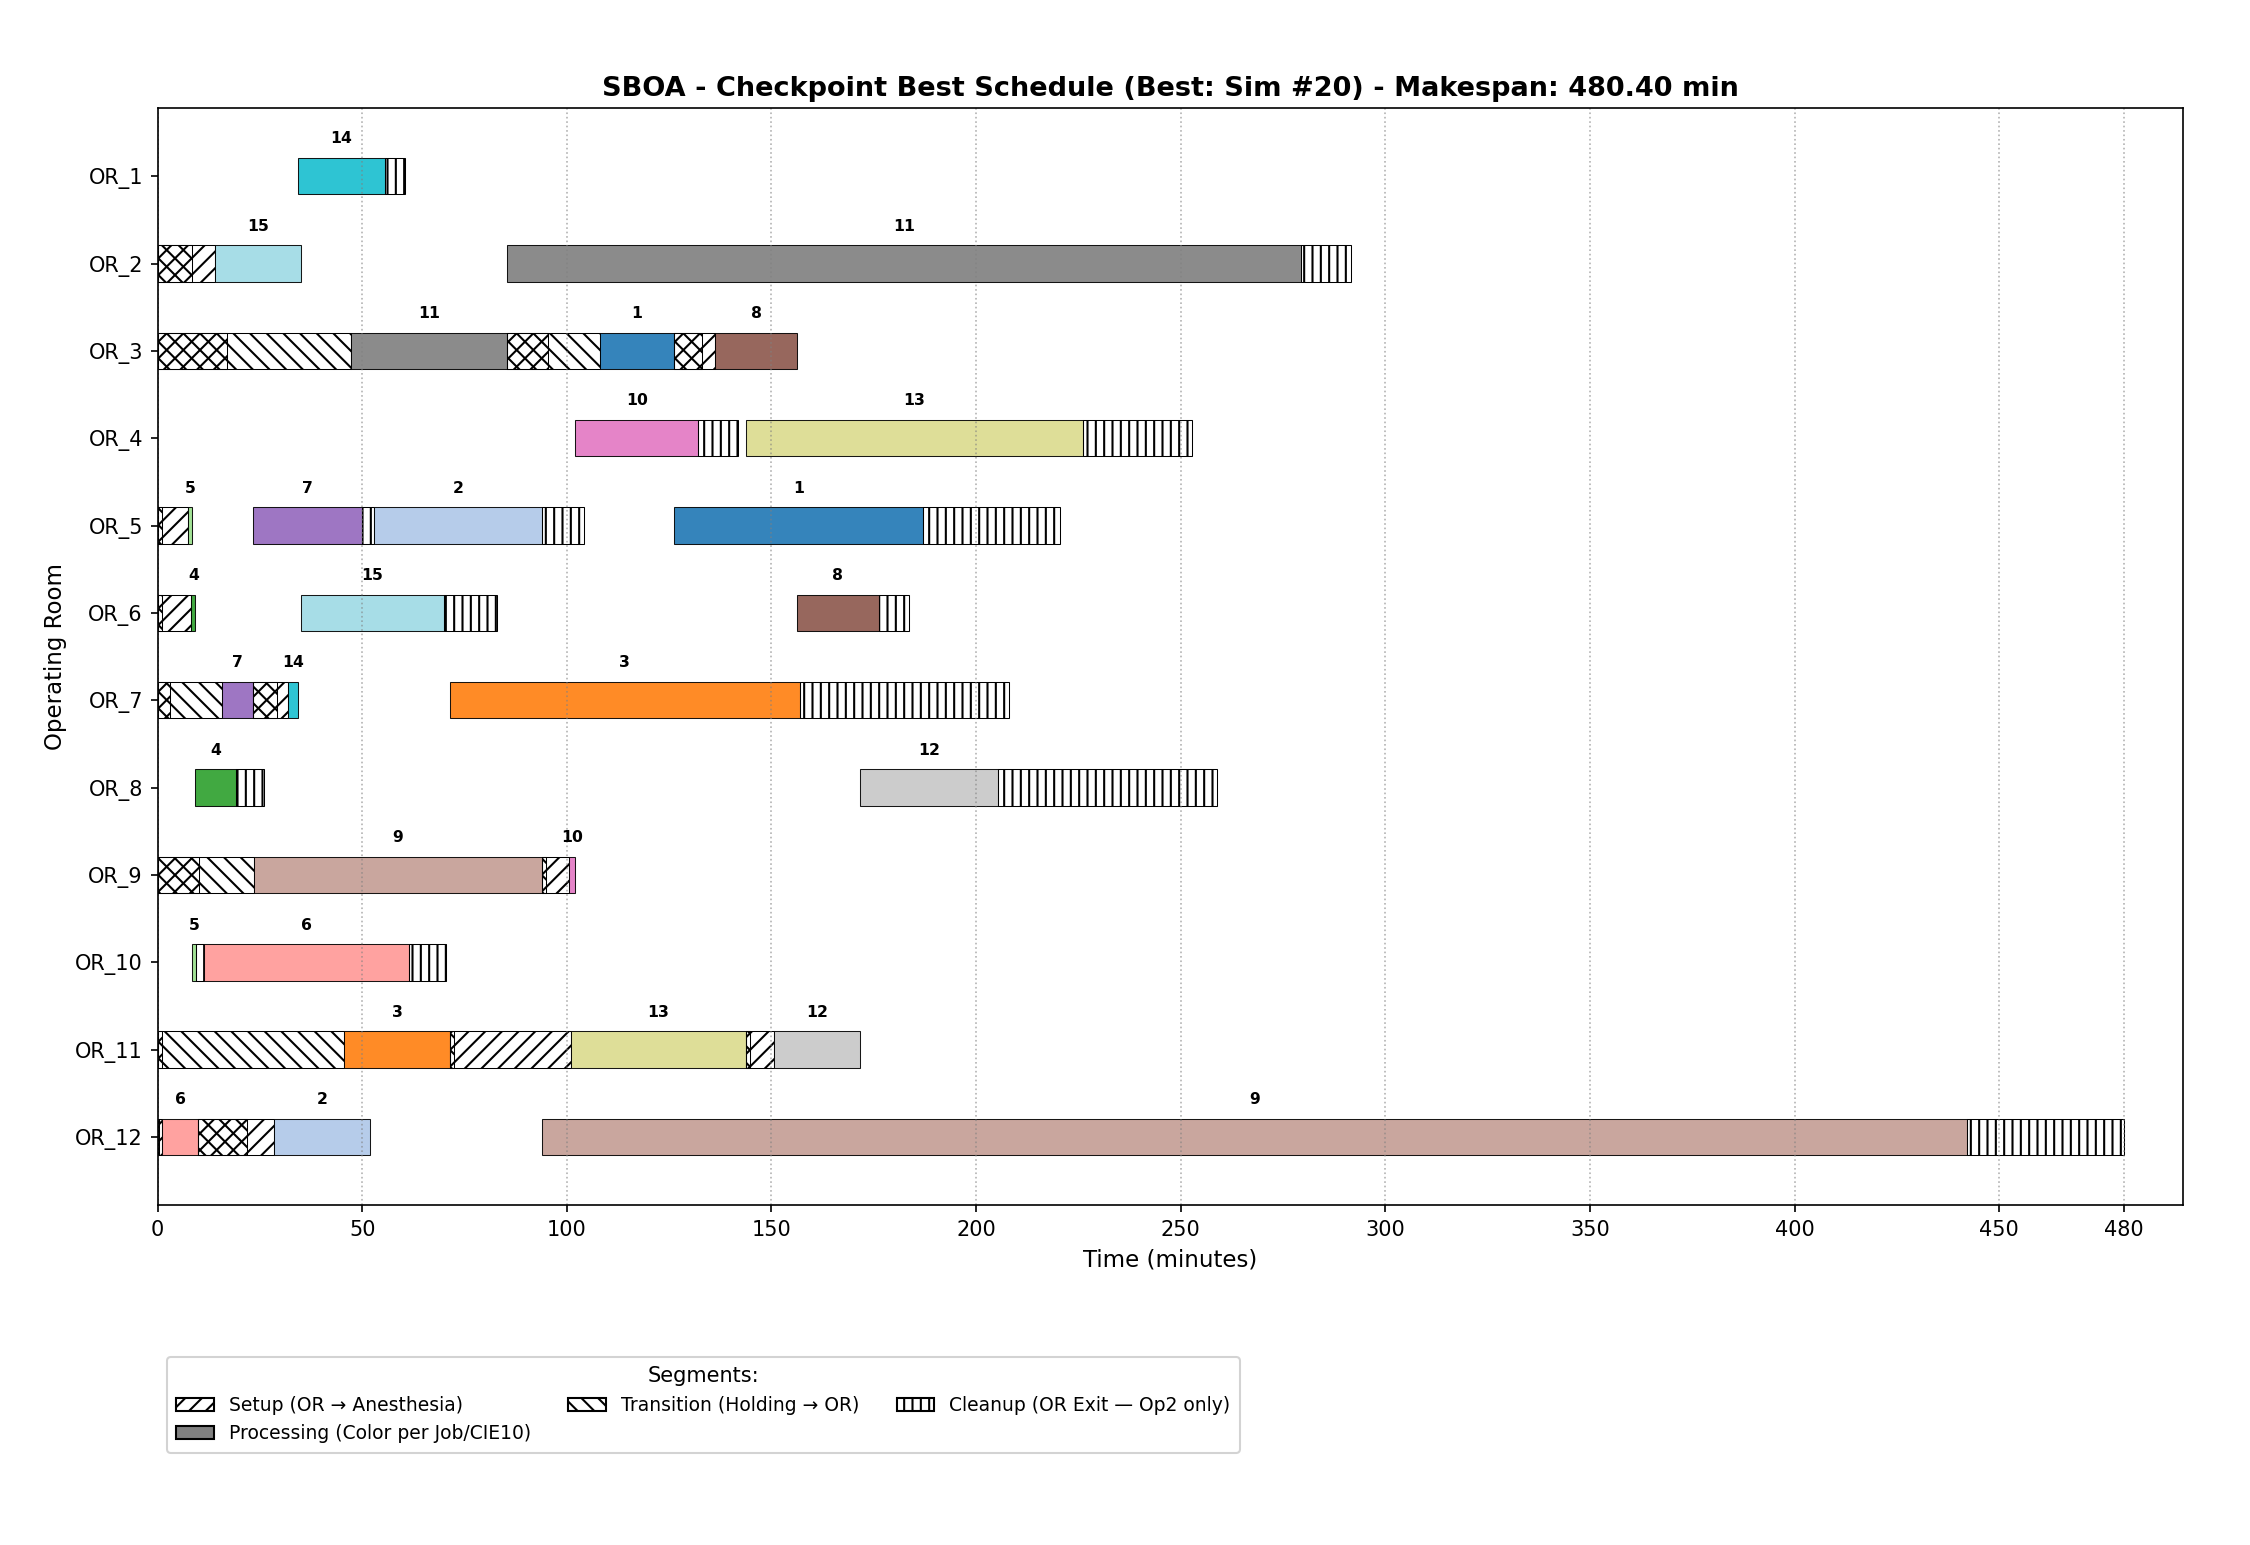
\includegraphics[width=\textwidth, height=0.83\textheight, keepaspectratio]{gantt_run1_sboa.png}
\end{frame}

%--------------------------------------------------------------
\begin{frame}{Baseline tradicional: regla constructiva FIFO (30 cirugías)}
  \centering
  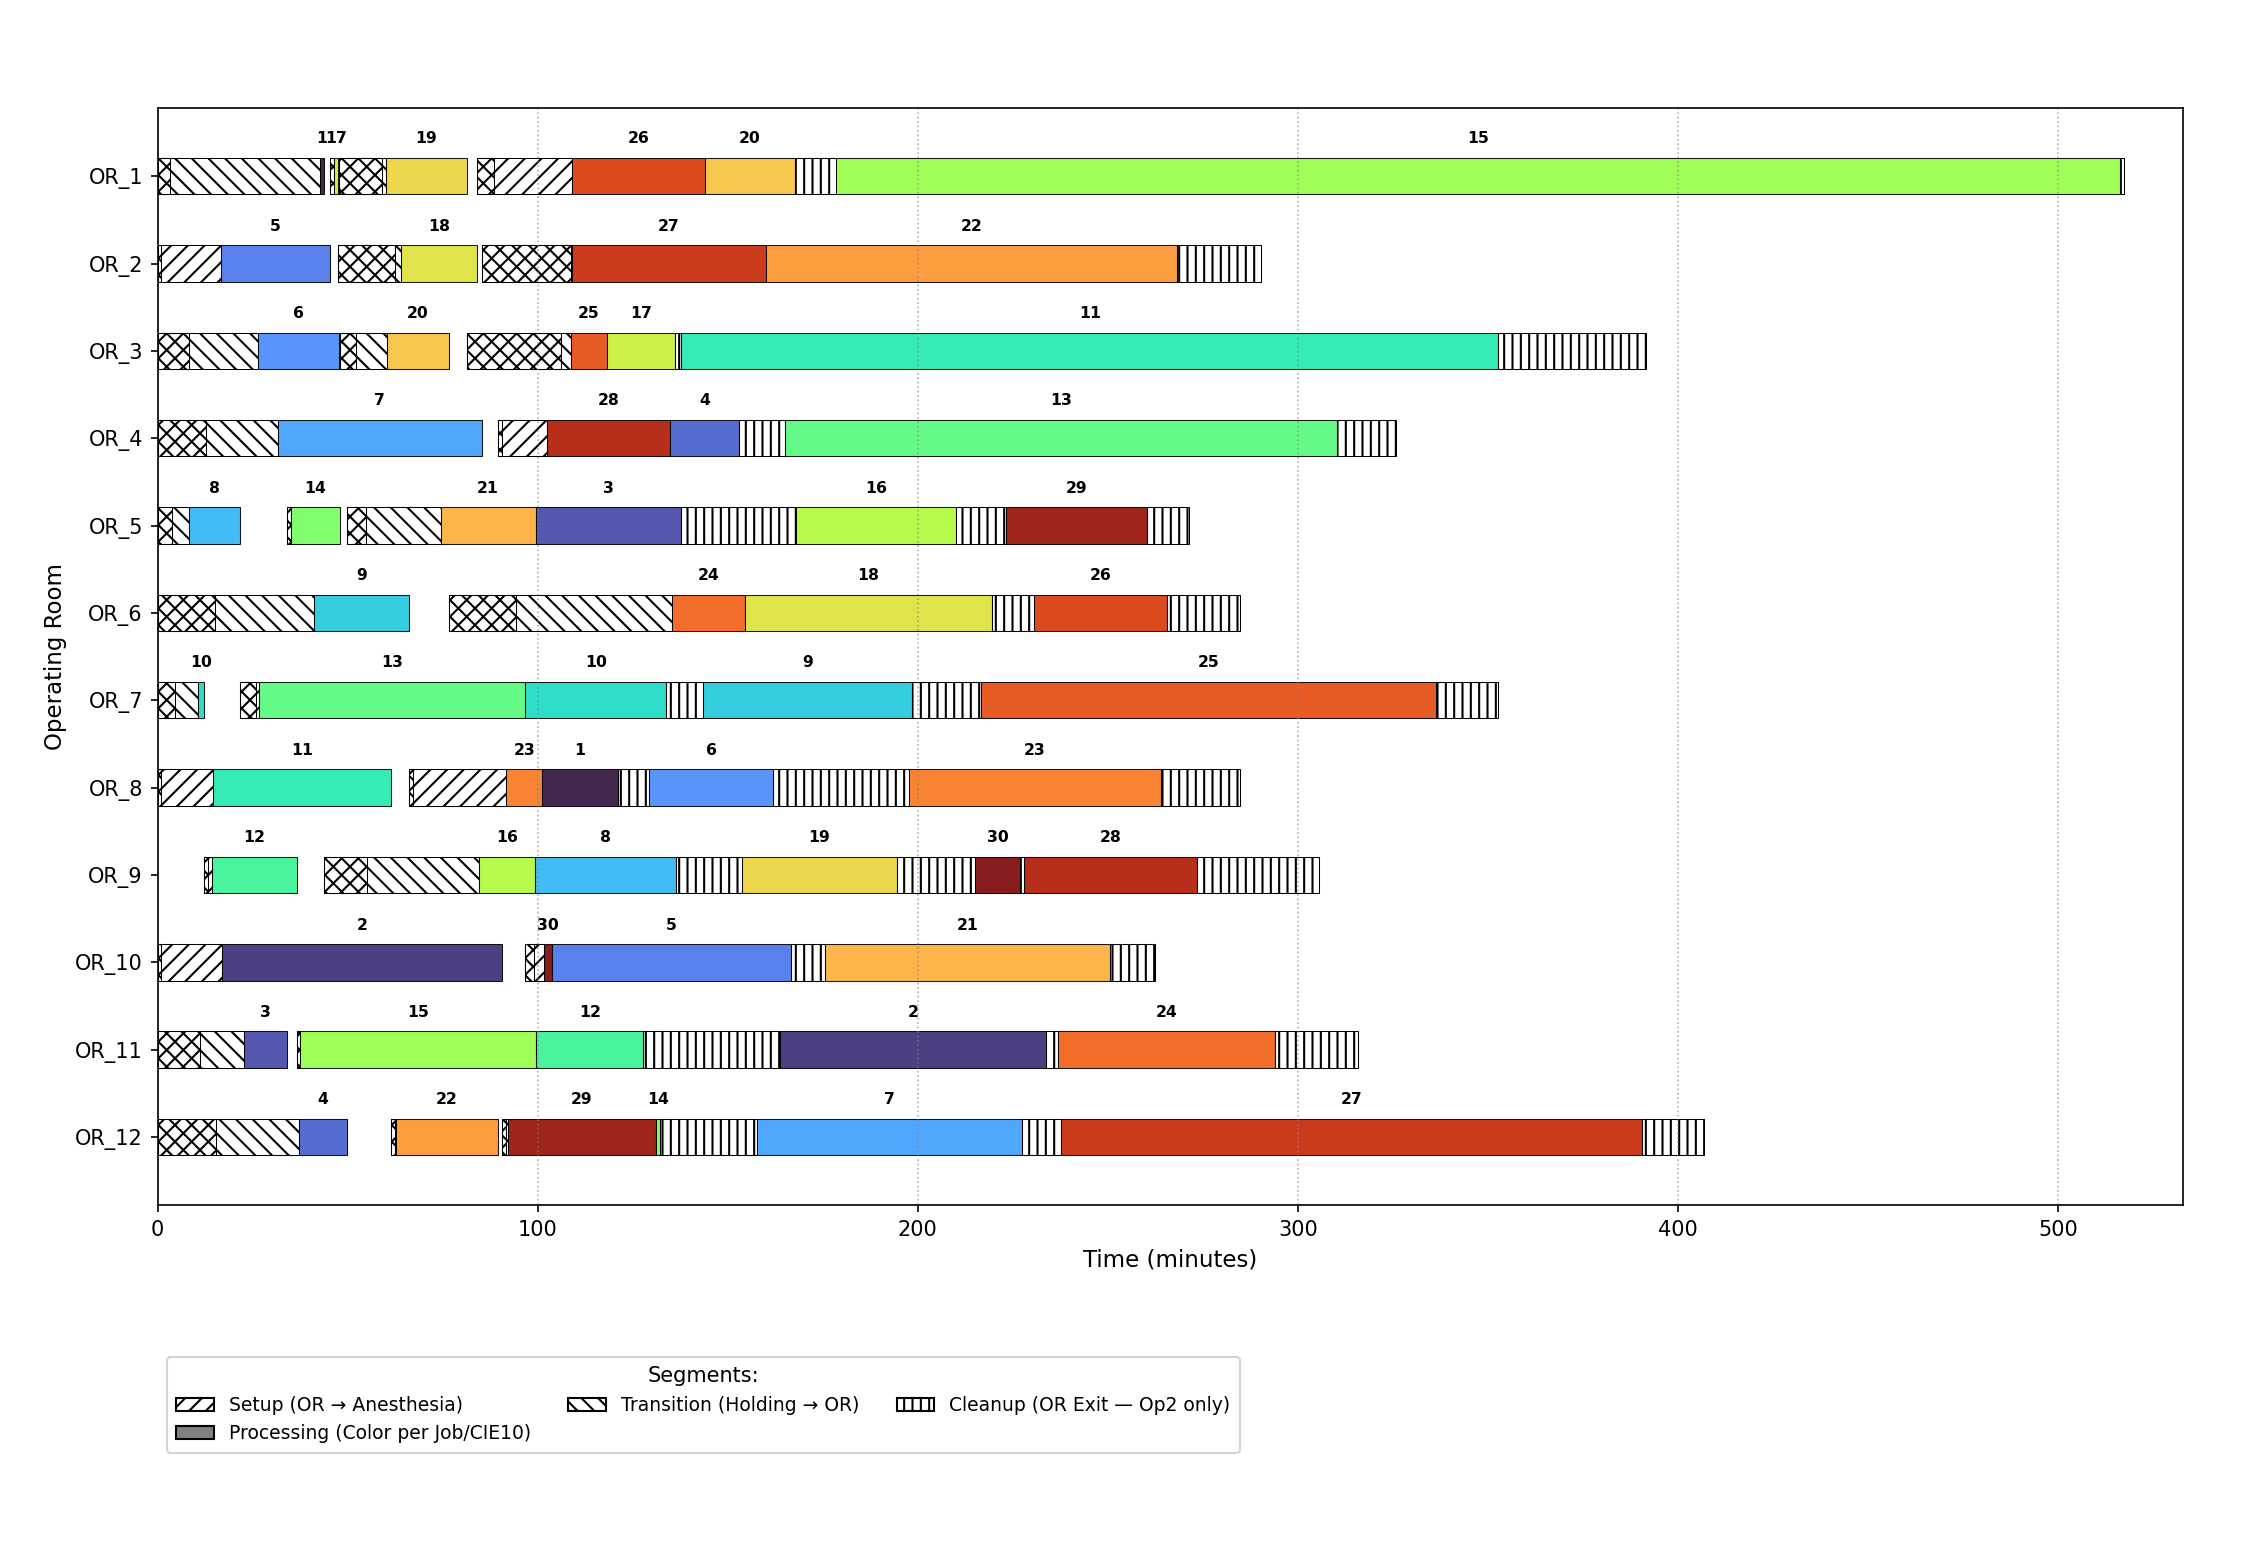
\includegraphics[width=\textwidth, height=0.83\textheight, keepaspectratio]{gantt_fifo_run4.png}
\end{frame}

%--------------------------------------------------------------
\begin{frame}{Resultado optimizado: metaheurística (30 cirugías)}
  \centering
  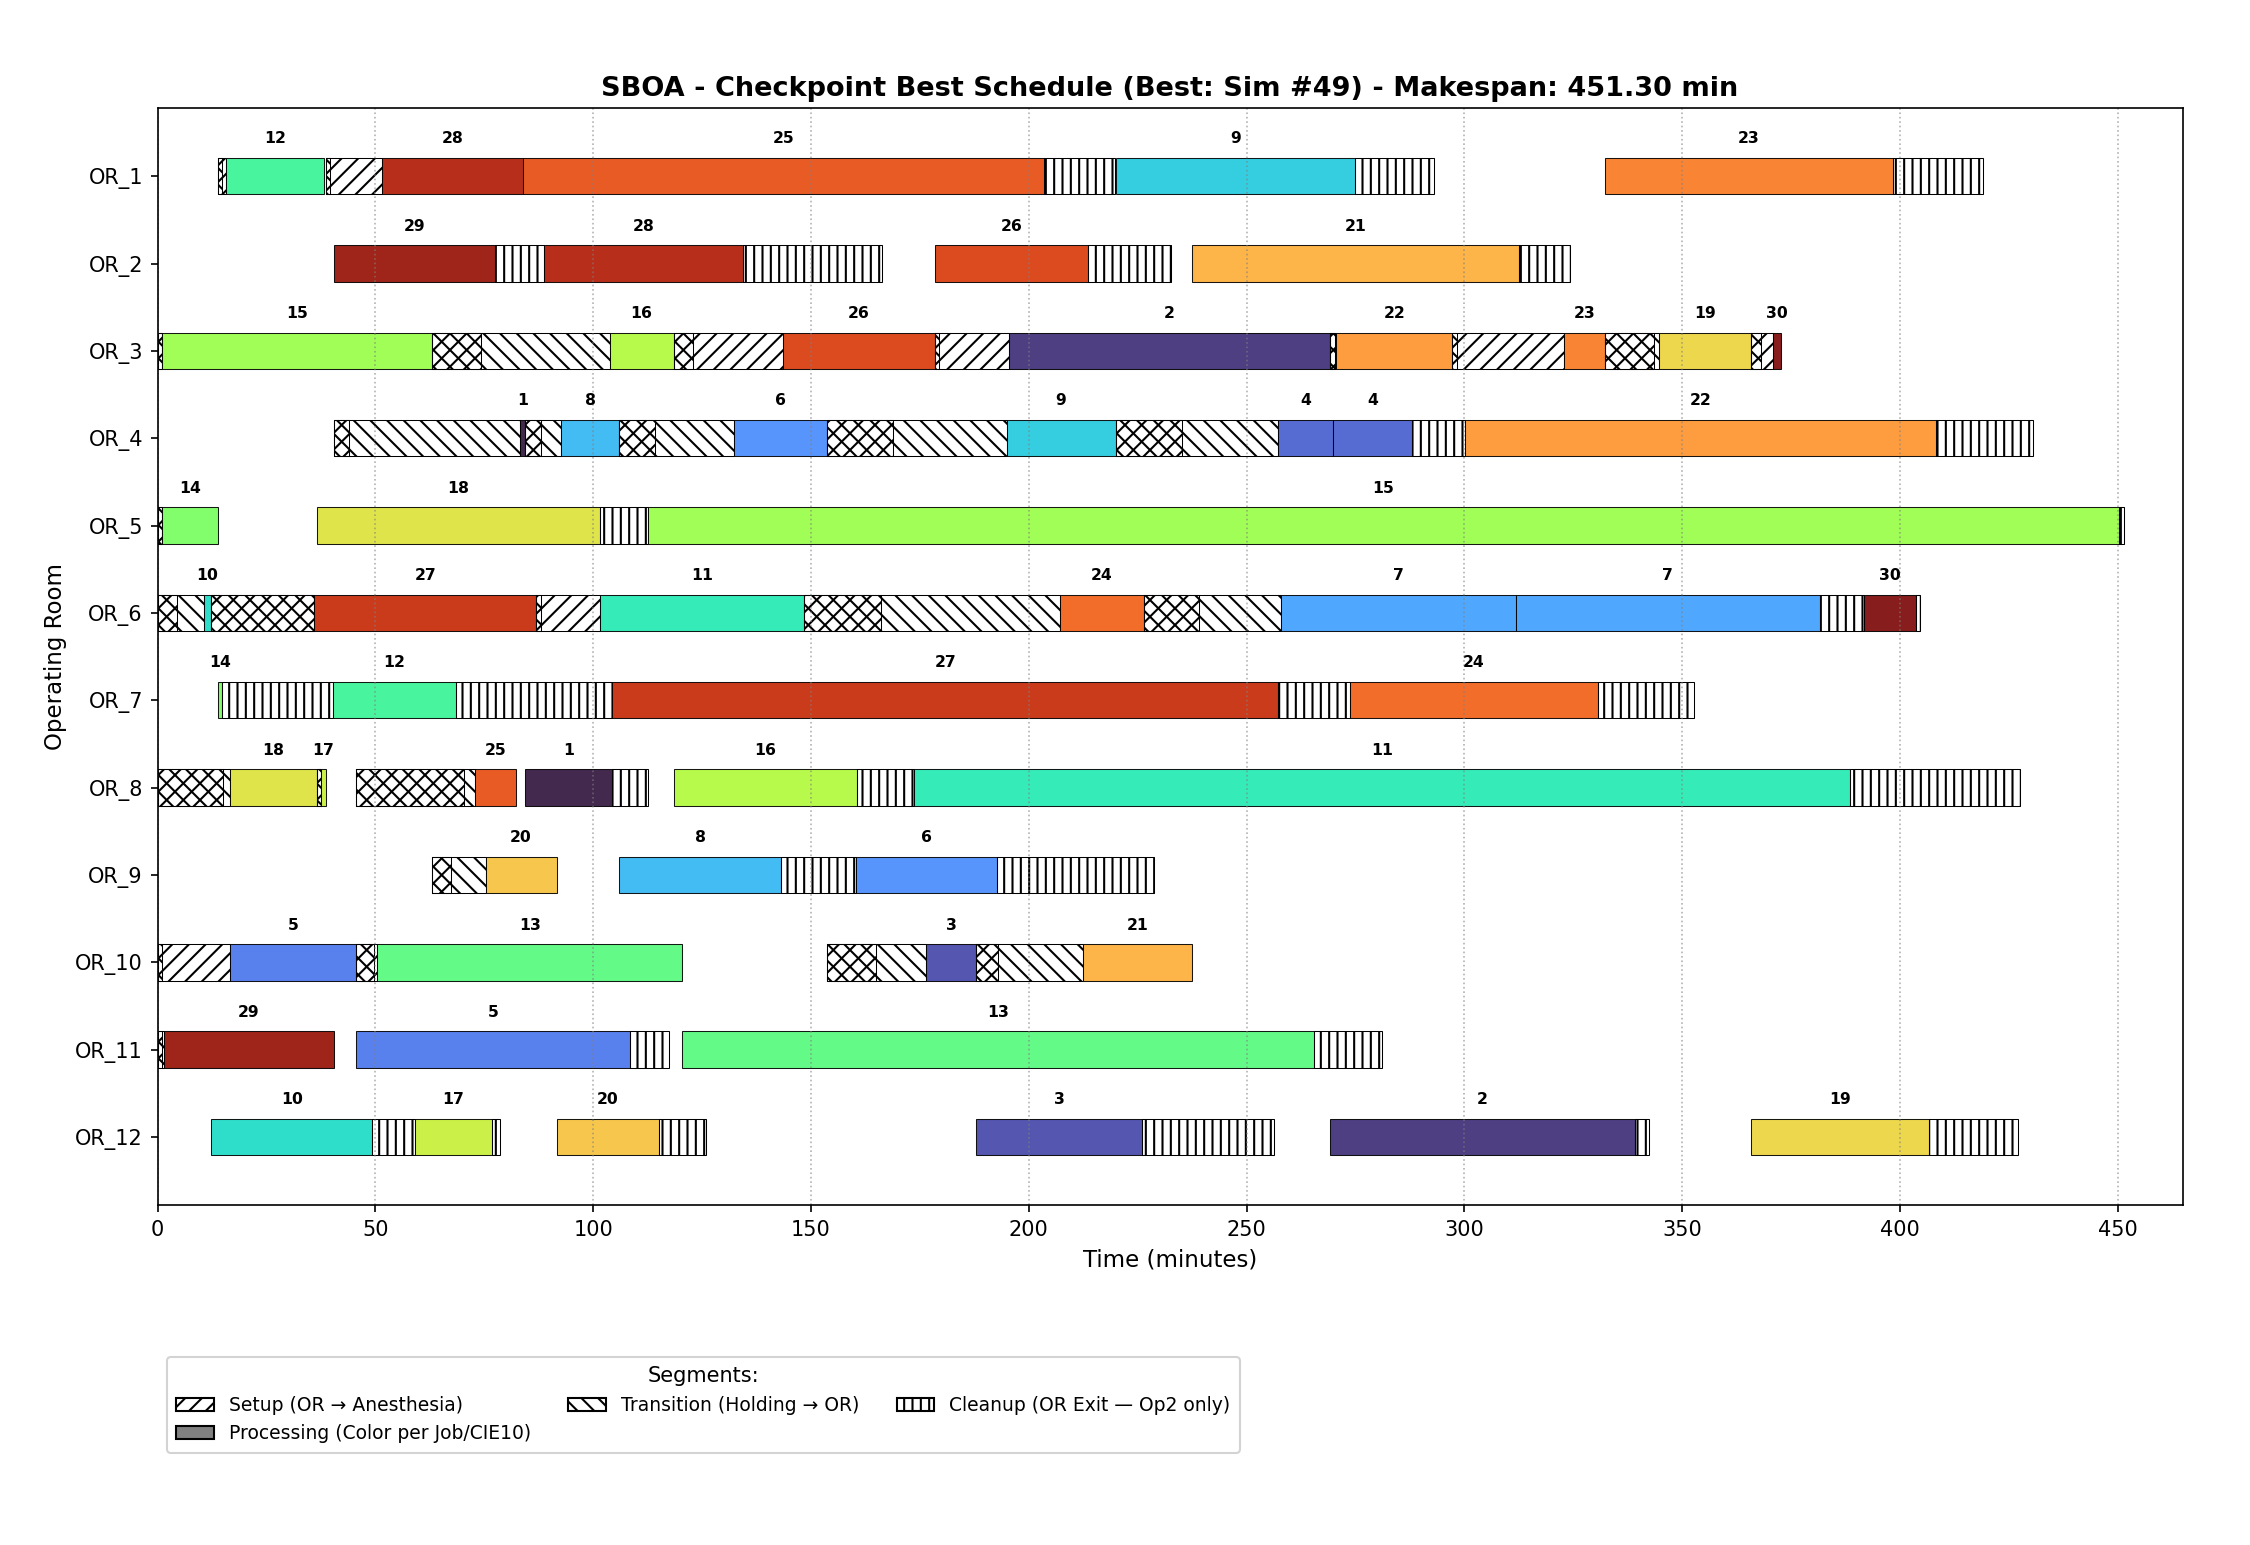
\includegraphics[width=\textwidth, height=0.83\textheight, keepaspectratio]{gantt_run4_sboa.png}
\end{frame}

%--------------------------------------------------------------
\begin{frame}{El desafío: pon a prueba tu metaheurística}
  \begin{columns}[t]
    \begin{column}{0.48\textwidth}
      \textbf{\color{primary}Starter Kit disponible:}
      \small
      \begin{itemize}
        \item \textbf{Instancias en JSON:} Instancias de \textbf{15, 20, 25 y 30 cirugías}, con diferentes tiempos de \textbf{anestesia}, \textbf{cirugía}, \textbf{setup}, \textbf{transición} y \textbf{limpieza}.
        \item \textbf{Simulador:} Evalúa la solución propuesta, calcula la función objetivo $f(S)$ y genera el gráfico de Gantt.
        \item \textbf{Baselines incluidos:} Reglas clásicas (FIFO, SPT y LPT) listas para comparar resultados.
      \end{itemize}
    \end{column}

    \begin{column}{0.52\textwidth}
      \begin{exampleblock}{El reto del taller}
        \small
        \begin{enumerate}
          \item \textbf{Conectar su algoritmo:} Integrar una metaheurística (GA, PSO, Tabu Search, SA, etc.).
          \item \textbf{Optimizar:} Reducir el Makespan y evitar que los quirófanos queden bloqueados.
          \item \textbf{Superar los baselines:} Mejorar los resultados de las reglas clásicas en las 4 instancias.
        \end{enumerate}
      \end{exampleblock}
    \end{column}
  \end{columns}
\end{frame}

%--------------------------------------------------------------
\begin{frame}[c]{Repositorio en GitHub}
  \vfill
  \centering
  \begin{minipage}{0.85\textwidth}
    \begin{block}{Código fuente, simulador e instancias}
      \centering\vspace{0.25cm}
      {\large\color{primary}\textbf{\url{https://github.com/Saicooh/OII464_Hospitales}}}
      \vspace{0.25cm}
    \end{block}
  \end{minipage}
  \vfill
\end{frame}

\end{document}